%This is a test file to determine the layout of the Owl Datasheet
\documentclass{article}
\pagestyle{myheadings}
\markright{BBa\_K783067}
\usepackage[xcolor]{mdframed} %Top header has banner!
\usepackage{hyphenat} %Column titles are not to have hyphenation
\usepackage{seqsplit} %Manages long DNA sequence line breaks
\usepackage{ccaption} %Formatting table titles
\usepackage[margin=1in]{geometry} %Setting document margins
\usepackage{graphicx} %Using images
\usepackage{array} %Formatting table size and behavior
\begin{document}
\renewcommand{\topfraction}{0.99} %Helps with keeping whitespace to a minimum
\renewcommand{\textfraction}{0.99}
\renewcommand{\floatpagefraction}{0.99}
\begin{table}[htbp]
\setlength{\belowcaptionskip}{4pt}
\setlength{\extrarowheight}{8pt}
\begin{mdframed}[backgroundcolor=gray!32,topline=false,rightline=false,leftline=false,bottomline=false] \legend{\Huge \underline{BBa\_K783067}} \end{mdframed} \hfill \break
\begin{tabular}{m{1.2in}m{4.98in}}
\large \textbf{\nohyphens{Summary}} & This is an inverter with pBad driving tetR with GFP as a reporter. pTetR has RFP has a reporter. We used a weaker RBS (B0032) to control the tetR expression and it helped the inverter function properly. We used flow cytometry to measure the function of our inverter. As arabinose concentration increases, tetR and GFP also increases. As the tetR amount increases, the RFP decreases as tetR represses the pTetR promoter controlling RFP.\\
\large \textbf{\nohyphens{Part Type}} & Composite Part\\
\large \textbf{\nohyphens{Pigeon Image}} & \hfill \break 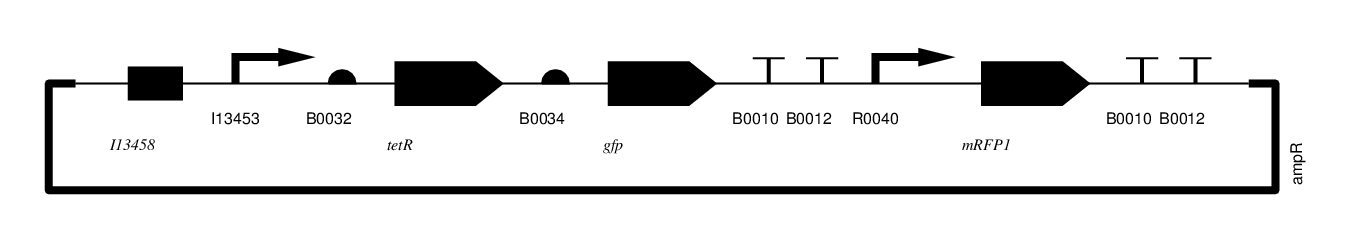
\includegraphics[width=10cm,height=10cm,keepaspectratio]{/Users/Zach/Documents/Owl/igem-datasheet/Datasheet_Generator/src/main/webapp/tmp/1439916870205BBa_K783067_pigeon.png} \
\end{tabular}
\end{table}
\begin{table}[htbp]
\setlength{\belowcaptionskip}{4pt}
\setlength{\extrarowheight}{8pt}
\begin{mdframed}[backgroundcolor=gray!32,topline=false,rightline=false,leftline=false,bottomline=false] \legend{\LARGE Designer Information}\end{mdframed}
\begin{tabular}{m{1.2in}m{4.98in}}
\large \textbf{\nohyphens{Author(s)}} & Traci Haddock\\
\large \textbf{\nohyphens{Data Collectors}} & Traci Haddock\\
\large \textbf{\nohyphens{Date}} & \seqsplit{2012}\\
\large \textbf{\nohyphens{Affiliation}} & Boston University\\
\large \textbf{\nohyphens{Team}} & \seqsplit{BostonU}\\
\large \textbf{\nohyphens{Contact}} & Traci Haddock
\end{tabular}
\end{table}
\begin{table}[htbp]
\setlength{\belowcaptionskip}{4pt}
\setlength{\extrarowheight}{8pt}
\begin{mdframed}[backgroundcolor=gray!32,topline=false,rightline=false,leftline=false,bottomline=false] \legend{\LARGE Designer Details}\end{mdframed}
\begin{tabular}{m{1.2in}m{4.98in}}
\large \textbf{\nohyphens{Type}} & GFP Reporter\\
\large \textbf{\nohyphens{Vector}} & \seqsplit{pSB1C3}\\
\large \textbf{\nohyphens{Design Components}} & \seqsplit{pBad-pTetR}
\end{tabular}
\end{table}
\begin{table}[htbp]
\setlength{\belowcaptionskip}{4pt}
\setlength{\extrarowheight}{8pt}
\begin{mdframed}[backgroundcolor=gray!32,topline=false,rightline=false,leftline=false,bottomline=false] \legend{\LARGE Assembly Information}\end{mdframed}
\begin{tabular}{m{1.2in}m{4.98in}}
\large \textbf{\nohyphens{Assembly Method(s)}} & \seqsplit{biobrick}\\
\large \textbf{\nohyphens{Chassis}} & e. coli\\
\large \textbf{\nohyphens{Assembly RFC}} & 10 and 23\\
\large \textbf{\nohyphens{Strain}} & bioline gold alpha\\
\large \textbf{\nohyphens{Scars}} & \seqsplit{y}
\end{tabular}
\end{table}
\begin{table}[htbp]
\setlength{\belowcaptionskip}{4pt}
\setlength{\extrarowheight}{8pt}
\begin{mdframed}[backgroundcolor=gray!32,topline=false,rightline=false,leftline=false,bottomline=false] \legend{\LARGE Flow Cytometry Experiment}\end{mdframed}
\begin{tabular}{m{1.2in}m{4.98in}}
\large \textbf{\nohyphens{Transfer Curve Graph}} & \hfill \break 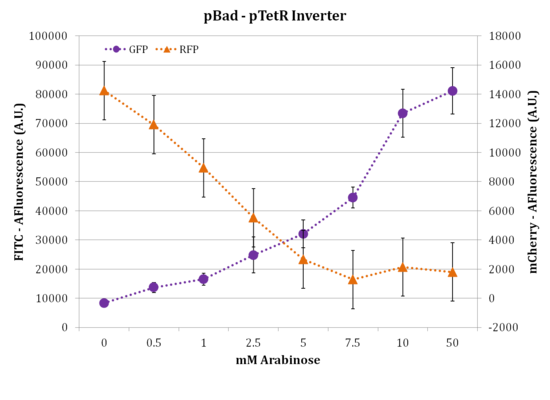
\includegraphics[width=10cm,height=10cm,keepaspectratio]{/Users/Zach/Documents/Owl/igem-datasheet/Datasheet_Generator/src/main/webapp/tmp/1439916870277BBa_K783067_transfer_curve.png} \
\end{tabular}
\end{table}
\end{document}
